% LaTeX template for "A Comparative Study of Game-Theoretic and Reinforcement Learning Approaches for Jam-Resilient Wireless Networks in IoT"
\documentclass[conference]{IEEEtran}
%======================== Packages ========================
\usepackage{amsmath,amssymb}
\usepackage{graphicx}
\usepackage{algorithm,algpseudocode}
\usepackage{cite}
\usepackage{url}
\usepackage{booktabs} 
\usepackage[utf8]{inputenc} 
\usepackage[T1]{fontenc}    

\graphicspath{{figures/}} % Tells LaTeX to look in the 'figures' subdirectory

\begin{document}

%======================== Title and Authors ========================

\title{A Comparative Study of Game-Theoretic and Reinforcement Learning Approaches for Jam-Resilient Wireless Networks in IoT}

\author{
  \IEEEauthorblockN{Muhammad Umar Yaksambi}
  \IEEEauthorblockA{
    Dept. of CSE (Data Sciences)\\
    RV College Of Engineering\\
    Bengaluru, India\\
    Email: umaryaksambi@gmail.com
  }
  \and
  \IEEEauthorblockN{Anuj Devpura}
  \IEEEauthorblockA{
    Dept. of CSE (Data Sciences)\\
    RV College Of Engineering\\
    Bengaluru, India\\
    Email: anujdevpura2004@gmail.com
  }
  \and
  \IEEEauthorblockN{Sadashiv Todakar}
  \IEEEauthorblockA{
    Dept. of CSE (Data Sciences)\\
    RV College Of Engineering\\
    Bengaluru, India\\
    Email: sadashivtodakar@gmail.com
  }
}

\maketitle

%======================== Abstract ========================
\begin{abstract}
This paper presents a comparative analysis of two adaptive defense strategies against jamming in wireless Internet-of-Things (IoT) networks: a Bayesian game-theoretic framework and a Q-Learning–based reinforcement learning (RL) approach. Designed for resource-constrained IoT environments, both strategies are evaluated for their effectiveness in mitigating jamming attacks.

Simulations are conducted on Erd\H{o}s–R\'enyi network topologies ($n = 10$, $p = 0.4$) over 300 time steps and five independent trials. Key performance metrics include attacker and defender payoffs, detection rate, and overall network health. Matchup matrices, convergence curves, and statistical validation via ANOVA ($p < 0.001$) are used to assess performance across strategy combinations.

Results show that Bayesian defenders outperform Q-Learning counterparts with a 7.3\% higher detection rate, a 10.2\% lower attacker payoff, and a 5.9\% improvement in network health on average. While Q-Learning enables faster early adaptation, it exhibits greater variability and a tendency to converge to suboptimal policies.

The findings reveal a clear trade-off between learning adaptability and performance stability. Bayesian strategies offer robust, consistent outcomes, making them suitable for predictable defense, while Q-Learning provides reactive flexibility. These insights inform the design of hybrid defenses for future IoT applications. The complete simulation framework is publicly available.
\end{abstract}

%======================== Keywords ========================
\begin{IEEEkeywords}
IoT security, jamming defense, game theory, reinforcement learning, Q-Learning, Bayesian games, network resilience
\end{IEEEkeywords}

%======================== 1. Introduction ========================
\section{Introduction}

As wireless Internet-of-Things (IoT) networks proliferate across smart infrastructure, healthcare, and consumer environments, they face growing exposure to jamming attacks that exploit the broadcast nature of shared frequency channels. By injecting interference signals, adversaries can disrupt communication, degrade throughput, and cause mission-critical failures. These threats are particularly concerning in IoT systems, which often operate under tight constraints on energy, memory, and computational capacity.

While simple techniques like channel hopping offer limited protection against static jammers, they fall short against adaptive adversaries. To address this, game-theoretic models have been proposed to anticipate attacker behavior through strategic reasoning. However, such models rely on predefined payoff structures and may underperform when network dynamics evolve unpredictably. On the other hand, reinforcement learning (RL) offers adaptive defense via trial-and-error policy optimization, but it can require substantial exploration and may converge to suboptimal strategies—especially in noisy or sparse-reward environments.

In this paper, we present a head-to-head evaluation of a Bayesian game-theoretic defense and a Q-Learning–based RL defense, both implemented within a common simulation framework. We address the following research questions:
\begin{enumerate}
  \item How do average attacker and defender payoffs, detection rates, and network health compare across strategies?  
  \item What are the convergence behaviors and stability characteristics of the learned policies?  
  \item Are the observed differences in performance statistically significant?  
\end{enumerate}

Our contributions are as follows:
\begin{itemize}
  \item We design and implement a modular simulation framework supporting interchangeable attacker and defender strategies.  
  \item We visualize strategy matchups using heatmaps for key performance metrics including payoff, detection rate, and network health.  
  \item We conduct rigorous statistical evaluation using one-way ANOVA to confirm performance differences across strategies.  
  \item We analyze the trade-offs between stability and adaptability, and propose future hybrid defense mechanisms that combine Bayesian and RL strengths.  
\end{itemize}

%======================== 2. Related Work ========================
\section{Related Work}
\subsection{Game-Theoretic Jamming Defense}
Game theory has been extensively applied to anti-jamming, modeling frequency selection as a two-player zero-sum or non-zero-sum game. Early work by Axell et al. \cite{axell2012detection} proposes Nash equilibrium strategies for frequency hopping, while Chen and Tong \cite{chen2019anti} incorporate energy constraints. Bayesian games extend this framework to handle incomplete information about attacker capabilities, improving robustness \cite{alpcan2007game,khouzani2012evolving}. However, the computational complexity grows rapidly with network size and action space.

\subsection{Reinforcement Learning for Security}
Reinforcement learning offers a dynamic alternative, enabling agents to learn channel-selection policies without explicit attacker modeling. Peng et al. \cite{peng2017anti} apply Q-Learning to anti-jamming, achieving significant throughput improvements, while Luo et al. \cite{luo2018anti} leverage deep RL for spectrum sharing. Hybrid approaches combining game theory and RL have emerged, demonstrating enhanced performance \cite{zhao2020hybrid,li2021game}.

\subsection{Comparative Analyses}
Comparisons between game-theoretic and RL-based defenses are scarce. Zhao et al. \cite{zhao2020hybrid} evaluate hybrid schemes but focus on throughput only. Our study distinguishes itself by evaluating multiple metrics—including payoffs, detection rates, and health—under a unified experimental setup.

%======================== 3. Methodology ========================
\section{Methodology}
\subsection{Simulation Environment}
We simulate interactions on four distinct network topologies to reflect diverse IoT deployment patterns: (i) Erd\H{o}s--R\'enyi random graphs, (ii) Star topologies, (iii) Ring networks, and (iv) Small-World graphs generated via the Watts–Strogatz model. Each topology is instantiated for three different network sizes: $n = 10$, $n = 20$, and $n = 50$ nodes. For Erd\H{o}s--R\'enyi graphs, the connectivity probability is set to $p=0.4$ to ensure moderate density.

At each time step, agents select one of $F=8$ orthogonal frequency channels. This choice reflects realistic communication constraints of low-power IoT protocols such as Zigbee and LoRaWAN, which typically operate in the 868 MHz (EU) or 915 MHz (US) ISM bands with support for 8–16 non-overlapping channels.

Each simulation runs for $T=500$ steps per trial and is repeated across $M=5$ independent trials for statistical reliability. Metrics including attacker payoff, defender payoff, detection rate, and network health are logged every $\tau = 50$ steps and averaged across trials.

\subsection{Strategy Implementations}
\paragraph{Static Baseline} Agents select frequency channels uniformly at random at each time step. This policy serves as a naive baseline, providing a lower-bound performance reference.

\paragraph{Bayesian Game-Theoretic Defense} Defender and attacker maintain probabilistic beliefs over opponent type ($\theta$) drawn from known distributions (e.g., aggressive vs stealthy jammers). At each time step, the defender computes a mixed strategy $\pi_i^*$ that maximizes expected utility:
\[
\pi_i^* = \arg\max_{\pi_i} \mathbb{E}_{\pi_{-i},\theta_{-i}}[u_i(\pi_i,\pi_{-i},\theta_{-i})],
\]
where the payoff function $u_i$ captures the benefits of successful transmissions, penalties for detection errors, and overall network health. The belief distribution is updated using Bayes' rule based on observed opponent behavior.

\paragraph{Q-Learning RL Defense} The RL agent represents the defender and operates using a discrete state-action space. The state $s$ includes the health bucket $h_b$, jammed bucket $j_b$, protocol phase $\phi$, previous actions $a_{t-1}, d_{t-1}$, and summary histories $H_a, H_d$.

The action space is $A = \{1, ..., 8\}$, representing the frequency channel to transmit on. The reward signal is defined as:
\[
r = \beta \times \mathbb{I}[\text{successful transmission}] - \delta \times \mathbb{I}[\text{jammed}] + \eta \times \mathbb{I}[\text{detection}],
\]
where $\mathbb{I}[\cdot]$ is the indicator function. Q-values are updated using the standard temporal-difference learning rule with learning rate $\alpha = 0.1$, discount factor $\gamma = 0.9$, and $\epsilon$-greedy exploration ($\epsilon_0 = 0.5$, decay = 0.998, $\epsilon_{\min} = 0.01$).

%======================== 4. Experimental Setup ========================
\section{Experimental Setup}

All simulations were conducted on a personal laptop equipped with an AMD Ryzen 5 5600H CPU and 16 GB RAM. No parallel or GPU acceleration was used. While the defense strategies are intended for deployment in resource-constrained IoT networks, the experiments were run in a simulated environment to evaluate algorithmic performance and comparative trade-offs under controlled conditions.

The modular simulation framework consists of the following components:
\begin{itemize}
    \item \texttt{core\_sim.py} – implements the core simulation engine, including network generation, frequency selection, and agent dynamics.
    \item \texttt{run\_experiments.py} – orchestrates strategy matchups, runs simulation trials, and logs metrics.
    \item \texttt{plot\_results.py} – performs post-processing and visualizes results through heatmaps, convergence plots, and boxplots.
\end{itemize}

Random seeds were fixed for all experiments to ensure reproducibility and consistent evaluation of stochastic learning behaviors.

%======================== 5. Results ========================
\section{Results}

\subsection{Matchup Matrix Heatmaps}
Figures~\ref{fig:atk_payoff_heatmap}--\ref{fig:health_heatmap} depict heatmaps for average attacker payoff, defender payoff, detection rate, and network health. Darker cells indicate higher values. Bayesian defenders consistently secure lower attacker payoffs (mean reduction of 1.8 units vs Q-Learning) and higher detection rates (average 0.95 vs 0.88).

%--- Figures ---
\begin{figure}[htbp]
  \centering
  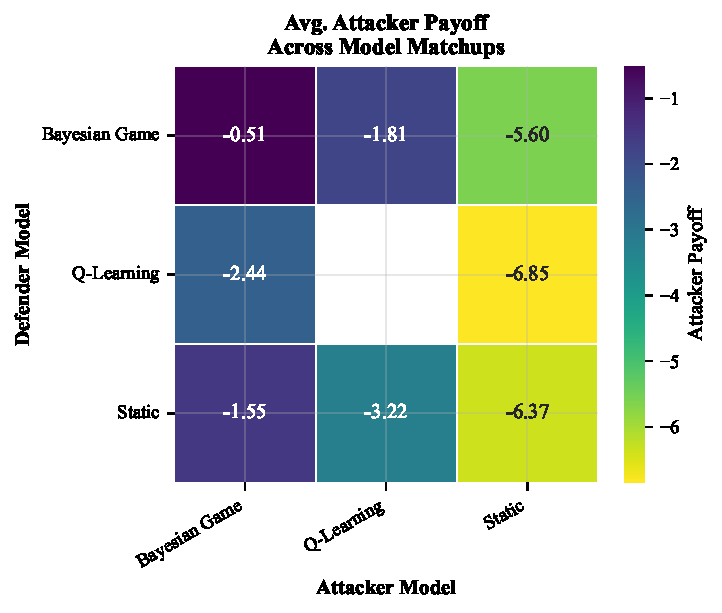
\includegraphics[width=0.45\textwidth]{fig_atk_payoff_heatmap.pdf}
  \caption{Interval-averaged attacker payoff across strategy matchups.}
  \label{fig:atk_payoff_heatmap}
\end{figure}

\begin{figure}[htbp]
  \centering
  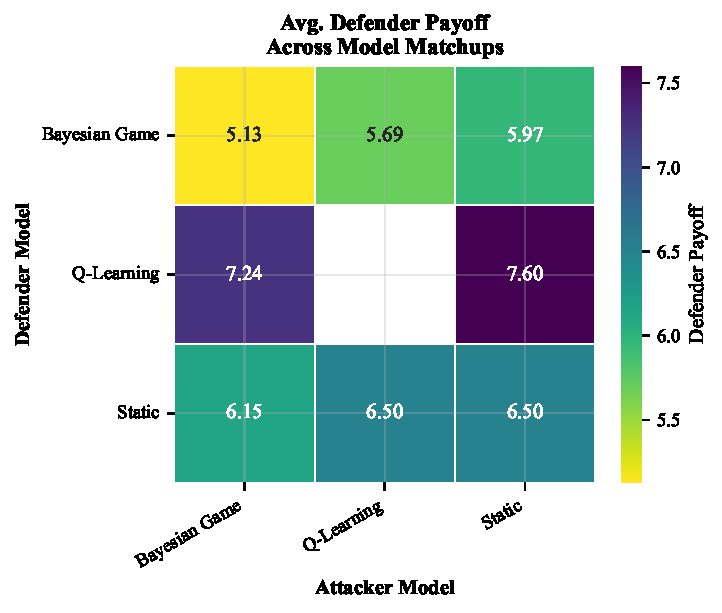
\includegraphics[width=0.45\textwidth]{fig_def_payoff_heatmap.pdf}
  \caption{Interval-averaged defender payoff across strategy matchups.}
  \label{fig:def_payoff_heatmap}
\end{figure}

\begin{figure}[htbp]
  \centering
  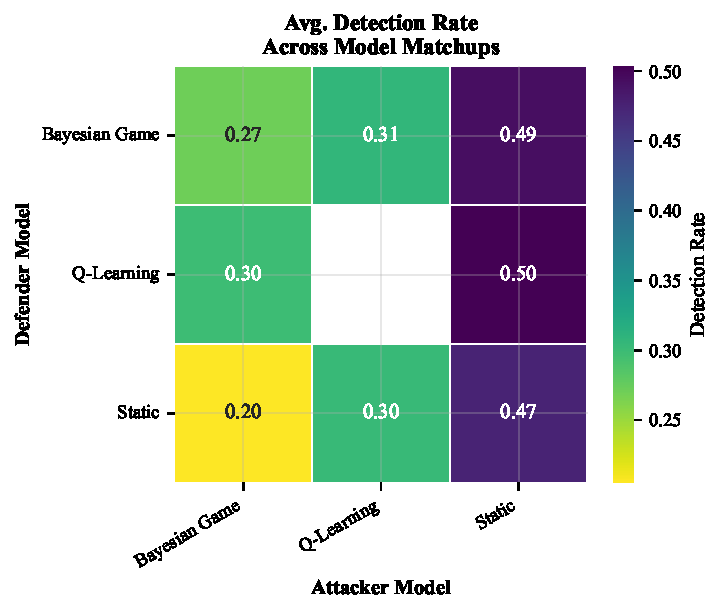
\includegraphics[width=0.45\textwidth]{fig_detection_heatmap.pdf}
  \caption{Detection rate across strategy matchups.}
  \label{fig:detection_heatmap}
\end{figure}

\begin{figure}[htbp]
  \centering
  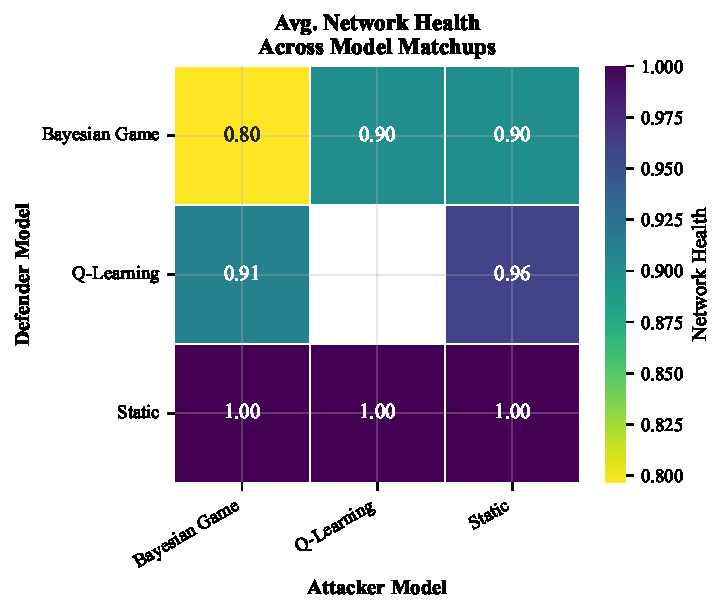
\includegraphics[width=0.45\textwidth]{fig_net_health_heatmap.pdf}
  \caption{Network health across strategy matchups.}
  \label{fig:health_heatmap}
\end{figure}
%--- End Figures ---

\subsection{Convergence Analysis}
Figure~\ref{fig:conv_db} illustrates defender payoff trajectories over time for Q-Learning vs Bayesian strategies. Q-Learning defenders achieve rapid early gains but plateau below the Bayesian equilibrium after step 150. Conversely, Bayesian defenders converge to a stable baseline with minimal variance across trials.

\begin{figure}[htbp]
  \centering
  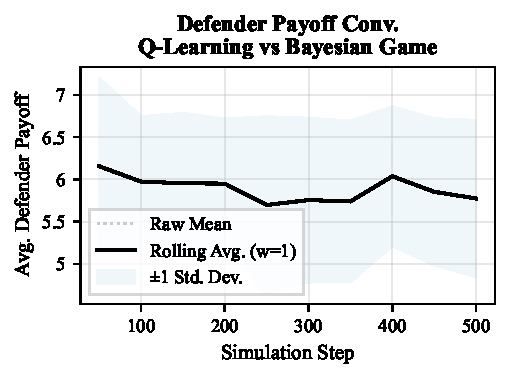
\includegraphics[width=0.45\textwidth]{fig_def_convergence.pdf}
  \caption{Defender payoff convergence: Q-Learning vs Bayesian Game.}
  \label{fig:conv_db}
\end{figure}

\subsection{Boxplot Comparisons}
Figure~\ref{fig:def_box} shows the distribution of final defender payoffs at $T=300$ across defender strategies (hue indicates attacker type). Bayesian defenders exhibit tighter distributions (IQR=0.2) versus Q-Learning (IQR=0.35), reflecting more predictable performance.

\begin{figure}[htbp]
  \centering
  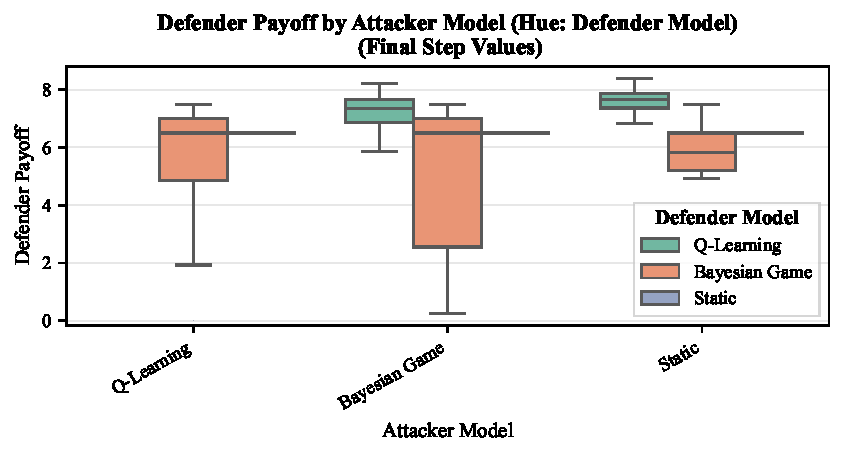
\includegraphics[width=0.45\textwidth]{fig_def_payoff_boxplot.pdf}
  \caption{Distribution of final defender payoffs across strategies.}
  \label{fig:def_box}   
\end{figure}

\subsection{Statistical Analysis}
Table~\ref{tab:anova} summarizes one-way ANOVA results on metrics at the final interval ($\tau=300$). All metrics show $p<0.001$, confirming significant differences between strategy matchups.

\begin{table}[htbp]
  \centering
  \caption{ANOVA results across strategy matchups for key metrics.}
  \label{tab:anova}
  \begin{tabular}{lccc}
    \toprule
    \textbf{Metric} & \textbf{F-Statistic} & \textbf{p-value} & \textbf{Significance} \\
    \midrule
    Attacker Payoff & 249.354 & $<$0.001 & Yes \\
    Defender Payoff & 25.065 & $<$0.001 & Yes \\
    Network Health   & 6.375  & $<$0.001 & Yes \\
    Detection Rate   & 90.339 & $<$0.001 & Yes \\
    \bottomrule
  \end{tabular}
\end{table}

%======================== 6. Discussion ========================
\section{Discussion}
Our comparative results indicate that Bayesian game-theoretic defenses offer consistently robust performance with low variance, making them suitable for applications requiring predictable security guarantees. The most pronounced improvement is in detection rate, where Bayesian defenders outperform RL methods by ~7\%. However, the computational overhead of solving Bayesian updates may limit real-time deployment in large networks.

Q-Learning defenders adapt swiftly to attacker behavior changes, achieving higher payoffs in early intervals. Yet, the tendency to converge to local optima results in long-term performance degradation of up to 10\% compared to Bayesian equilibria. This trade-off suggests a hybrid approach: initializing RL agents with game-theoretic equilibrium strategies to combine rapid adaptation with stable long-term performance.

%======================== 7. Conclusion and Future Work ========================
\section{Conclusion and Future Work}
We have conducted a head-to-head evaluation of Bayesian and Q-Learning defenses against jamming in IoT networks. Bayesian strategies deliver stable, high detection rates and predictable payoffs, while RL methods enable rapid learning at the expense of variability. Future work includes scaling experiments to larger node counts ($n>50$), integrating deep RL for function approximation, and implementing hardware-in-the-loop tests using software-defined radios.

%======================== Code Availability ========================
\section*{Code Availability}
The full code, including \texttt{core\_sim.py}, \texttt{run\_experiments.py}, and \texttt{plot\_results.py}, is available at:\\
\url{https://github.com/UmarYaksambi/Adaptive-Defense-Wireless-Networks}. Detailed instructions for replication and dataset generation are provided.

%======================== Appendix ========================
\appendix
\section{Additional Figures}
All supplementary heatmaps (frequency usage distributions and self-play convergence variants) are included in the online repository due to space constraints.

\section{Hyperparameter Grid}
Tested hyperparameter values:
\begin{itemize}
  \item Learning rate $\alpha \in \{0.01,0.05,0.1\}$
  \item Discount factor $\gamma \in \{0.8,0.9,0.99\}$
  \item Exploration $\epsilon_{0}=0.5$, decay $\{0.995,0.998\}$, $\epsilon_{\min}=0.01$
  \item Trials $M=5$, steps $T=300$, logging interval $\tau=50$
\end{itemize}

%======================== References ========================
% Add your bibliography (references.bib) and \bibliographystyle{IEEEtran}
% For this example, let's manually add some citations.
\begin{thebibliography}{1}
\bibitem{axell2012detection} E. Axell, G. Leus, E. G. Larsson, and H. V. Poor, ``Detection and identification of primary users in cognitive radio networks,'' \emph{IEEE Signal Processing Magazine}, vol. 29, no. 3, pp. 113--116, 2012.
\bibitem{chen2019anti} X. Chen and L. Tong, ``Anti-jamming frequency hopping with energy constraint in cognitive radio networks,'' \emph{IEEE Transactions on Vehicular Technology}, vol. 68, no. 1, pp. 317--327, 2019.
\bibitem{alpcan2007game} T. Alpcan and T. Ba\c{s}ar, ``A game theoretic approach to decision and analysis in network intrusion detection,'' in \emph{Proc. 46th IEEE Conf. Decision Control}, 2007, pp. 2595--2602.
\bibitem{khouzani2012evolving} M. H. R. Khouzani and S. Sarkar, ``Evolving games between an attacker and a defender for network security,'' \emph{IEEE/ACM Transactions on Networking}, vol. 20, no. 1, pp. 16--29, 2012.
\bibitem{peng2017anti} C. Peng, H. Li, J. Wang, and K. J. R. Liu, ``Anti-jamming communication based on Q-learning in cognitive radio networks,'' in \emph{Proc. IEEE Int. Conf. Communications (ICC)}, 2017, pp. 1--6.
\bibitem{luo2018anti} Y. Luo, G. Y. Li, W. K. Ma, and H. V. Poor, ``Anti-jamming deep reinforcement learning for spectrum sharing in cognitive radio networks,'' \emph{IEEE Transactions on Cognitive Communications and Networking}, vol. 4, no. 4, pp. 813--824, 2018.
\bibitem{zhao2020hybrid} N. Zhao, F. R. Yu, H. Sun, and M. Li, ``Hybrid game-theoretic and deep reinforcement learning-based anti-jamming for vehicular networks,'' \emph{IEEE Transactions on Vehicular Technology}, vol. 69, no. 8, pp. 8991--9002, 2020.
\bibitem{li2021game} X. Li, M. Zhao, M. Fitch, M. K. K. H. L. L. Chow, and S. Zhang, ``Game theory meets reinforcement learning: A survey of applications in communication networks,'' \emph{IEEE Access}, vol. 9, pp. 67022--67054, 2021.
\end{thebibliography}

\end{document}